\documentclass{report}
% Maths Packages
\usepackage{mathtools, amsthm, amssymb, mathrsfs, interval, stmaryrd, centernot, esvect, cancel, commath, blkarray, empheq}
\usepackage{tabularx}
\usepackage{booktabs}
\usepackage{cellspace}
\setlength{\cellspacetoplimit}{5pt}
\setlength{\cellspacebottomlimit}{5pt}

% Sagemaths Formating Packages
\usepackage{listings}
\lstdefinelanguage{Sage}[]{Python}
{morekeywords={False,sage,True},sensitive=true}
\lstset{
  frame=none,
  showtabs=False,
  showspaces=False,
  showstringspaces=False,
  commentstyle={\ttfamily\color{dgreencolor}},
  keywordstyle={\ttfamily\color{dbluecolor}\bfseries},
  stringstyle={\ttfamily\color{dgraycolor}\bfseries},
  language=Sage,
  basicstyle={\fontsize{10pt}{10pt}\ttfamily},
  aboveskip=0.4em,
  belowskip=0.4em,
}

% TOC Packages
\usepackage{tocloft, titletoc, hyperref, bookmark}
% Formatting / Style Packages
\usepackage[T1]{fontenc}
\usepackage{geometry, subcaption, graphicx, fix-cm, accents, float, varwidth, soul, ulem, contour, multicol, enumitem}    
\usepackage[bottom]{footmisc}
\usepackage[x11names, table]{xcolor}
\usepackage[most, skins]{tcolorbox}
\usepackage{adjustbox}
\DeclareMathAlphabet{\mathmybb}{U}{bbold}{m}{n} % Indicatrices
\newcommand{\1}{\mathmybb{1}}

% Tikz
\usepackage{tikz, tkz-fct, tkz-euclide, tikz-cd, tkz-fct, pgfplots}
\pgfplotsset{compat=1.18}
\usetikzlibrary{
  angles, quotes, 3d, positioning,
  shapes,fit, arrows, arrows.meta, calc, 
  matrix, calligraphy, intersections, 
  quotes, patterns, patterns.meta, 
  decorations.pathreplacing, decorations.markings,decorations.pathmorphing,
}
\usepgfplotslibrary{fillbetween}
\tikzset{
  withparens/.style = {draw, outer sep=0pt,
    left delimiter= (, right delimiter=),
    above delimiter= (, below delimiter=),
    align=center},
  withbraces/.style = {draw, outer sep=0pt,
    left delimiter=\{, right delimiter=\},
    above delimiter=\{, below delimiter=\},
    align=center}
}
\tikzcdset{
  arrow style=tikz,
  diagrams={>={Straight Barb[scale=1]}},
}

% PAGE SETTINGS

\geometry{
  left=25mm, right=25mm, top= 15mm, bottom= 15mm,
  footskip=30pt
  }
\setlength{\parindent}{0cm}
\setlength{\parskip}{0cm}
\setlist[itemize]{itemsep=0pt, leftmargin=25pt}

\setlength{\cftbeforetoctitleskip}{0pt}
\setlength{\cftaftertoctitleskip}{0pt}

\definecolor{BrightBlue1}{RGB}{95, 150, 210}

\definecolor{BrightRed1}{RGB}{210, 95, 95}
\definecolor{BrightRed2}{RGB}{210, 115, 115}

\definecolor{DarkBlueX}{RGB}{43, 68, 92}
\definecolor{DarkBlue0}{RGB}{53, 78, 102}
\definecolor{DarkBlue1}{RGB}{83, 108, 132}
\definecolor{DarkBlue2}{RGB}{58, 94, 132}
\definecolor{DarkBlue3}{RGB}{90, 126, 162}

\definecolor{DarkGreen3}{RGB}{83, 132, 108}
\definecolor{DarkGreen2}{RGB}{58, 132, 94}
\definecolor{DarkGreen1}{RGB}{90, 162, 126}
\tcbset{shield externalize, enhanced, sharp corners, halign=center, center}

\definecolor{dblackcolor}{rgb}{0.0,0.0,0.0}
\definecolor{dbluecolor}{rgb}{0.01,0.02,0.7}
\definecolor{dgreencolor}{rgb}{0.2,0.4,0.0}
\definecolor{dgraycolor}{rgb}{0.30,0.3,0.30}
\newcommand{\dblue}{\color{dbluecolor}\bf}
\newcommand{\dred}{\color{dredcolor}\bf}
\newcommand{\dblack}{\color{dblackcolor}\bf}

%Underline settings
\setlength{\ULdepth}{2pt}
\contourlength{0.8pt}
\renewcommand{\underline}[1]{
  \uline{\phantom{#1}}%
  \llap{\contour{white}{#1}}%
}

%drop shadow southwest=black!100!black
\newcommand{\secstyle}[1]{\color{DarkBlue1}\fbox{#1}}
\newcommand{\subsecstyle}[1]{\color{DarkBlue2}\underline{#1}}
\newcommand{\subsubsecstyle}[2]{\color{DarkBlue3}\underline{#1}}

\newcommand{\chapterstyle}[1]{
    \setlength{\fboxsep}{0.3em}
    \setlength{\fboxrule}{3pt}
    \centering\vspace{-70pt}
    
    \color{DarkBlue1}\huge\fbox{\textbf{\textsc{#1}}}
}

\newcommand{\customBox}[2]{
    \tcbset{boxrule=1.5pt, boxsep=-0.2mm, colframe=DarkBlue1, colback=BrightBlue1!05}
    \begin{tcolorbox}[#1]
        \abovedisplayskip=0pt % remove vertical space above align
        #2
    \end{tcolorbox}
}

\makeatletter % Crée une trés grosse taille de police pour la page de garde
\newcommand\HUGE{\@setfontsize\Huge{40}{60}}
\makeatother   

\makeatletter
\newcommand\footnoteref[1]{\protected@xdef\@thefnmark{\ref{#1}}\@footnotemark}
\makeatother
% TOC
\renewcommand{\cftchapfont}{\large \bfseries \scshape}
\renewcommand{\cftsecfont}{}
\renewcommand{\contentsname}{\hfill
\setlength{\fboxsep}{0.3em}\setlength{\fboxrule}{3pt}\vspace{20pt}
   \color{DarkBlue1}\Huge
   \fbox{\textbf{\textsc{Table des matières}}}
   \hfill
}

% MATHS
\newcommand{\C}{\mathbb{C}}
\newcommand{\R}{\mathbb{R}}
\newcommand{\Q}{\mathbb{Q}}
\newcommand{\Z}{\mathbb{Z}}
\newcommand{\N}{\mathbb{N}}
\newcommand{\U}{\mathbb{U}}
\newcommand{\K}{\mathbb{K}}

\newcommand{\A}{\mathbf{\mathscr{A}}}
\newcommand{\B}{\mathbf{\mathscr{B}}}
\newcommand{\Fam}{\mathbf{\mathscr{F}}}
\renewcommand{\P}{\mathbf{\mathscr{P}}}

\renewcommand{\epsilon}{\varepsilon}
\renewcommand{\rho}{\varrho}

\newcommand{\E}{\mathbf{\mathcal{E}}}
\newcommand{\F}{\mathbf{\mathcal{F}}}
\newcommand{\Pow}{\mathbf{\mathcal{P}}}
\newcommand{\G}{\mathbf{\mathfrak{G}}}

\newcommand{\<}{\bigskip}
\newcommand{\+}{\par}

% Notation equality

\newcommand\notationEq{\stackrel{\mbox{
    \begin{tiny}  
        notation
    \end{tiny}    
}}{=}}

% INTERVALS

\intervalconfig{separator symbol =  \,; \,}

\newcommand{\ioo}[2]{\interval[open]{#1}{#2}}
\newcommand{\ioc}[2]{\interval[open left]{#1}{#2}}
\newcommand{\ico}[2]{\interval[open right]{#1}{#2}}
\newcommand{\icc}[2]{\interval{#1}{#2}}

\newcommand{\intioo}[2]{\left\rrbracket{#1}\;;\;{#2}\right\llbracket}
\newcommand{\intioc}[2]{\left\rrbracket{#1}\;;\;{#2}\right\rrbracket}
\newcommand{\intico}[2]{\left\llbracket{#1}\;;\;{#2}\right\llbracket}
\newcommand{\inticc}[2]{\left\llbracket{#1}\;;\;{#2}\right\rrbracket}

% EQUATIONS NOTES

\newcommand{\shorteqnote}[1]{ &  & \text{\small\llap{#1}}}
\newcommand{\longeqnote}[1]{& & \\ \notag&  &  &  &  & \text{\small\llap{#1}}}

% FUNCTIONS NOTATIONS

\newcommand{\inject}{\hookrightarrow} 
\newcommand{\surject}{\twoheadrightarrow}

% MOD NOTATION

\newcommand{\eqmod}[1]{\underset{#1}{\equiv}} 

% LINEAR ALGEBRA

\newcommand{\dotproduct}[2]{\left\langle\;\! #1 \;\! | \;\! #2 \;\! \right\rangle}
\newcommand{\vectNorm}[1]{\left\Vert#1 \right\Vert}

\newcommand{\Ker}[1]{\text{Ker}#1}
\newcommand{\Sp}[1]{\text{Sp}(#1)}
\renewcommand{\Im}[1]{\text{Im}#1}

\NewDocumentCommand{\opNorm}{sO{}m}{%
  \IfBooleanTF{#1}{% automatic scaling, use with care
    \left|\opnormkern\left|\opnormkern\left|
    #3
    \right|\opnormkern\right|\opnormkern\right|
  }{
    \mathopen{#2|\opnormkern #2|\opnormkern #2|}
    #3
    \mathclose{#2|\opnormkern #2|\opnormkern #2|}
  }%
}
\newcommand{\opnormkern}{\mkern-1.5mu\relax}% adjust for the font

% TOPOLOGY
\newcommand{\ball}{\mathscr{B}}

% CALCULUS
\newcommand{\partialD}[2]{\frac{\partial #1}{\partial #2}}

% GEOMETRY
\newcommand{\RightAgnle}[4][5pt]
{%
    \draw($#3!#1!#2$)-- ($#3!2! ($ ($#3!#1!#2$)!.5! ($#3!#1!#4$)$)$)-- ($#3!#1!#4$);
}

% PROBABILITIES
\newcommand{\probability}[1]{\mathbb{E} (#1)}
\newcommand{\expectancy}[1]{\mathbb{E} (#1)}
\newcommand{\variance}[1]{\mathbb{V} (#1)}
\newcommand{\covariance}[1]{\mathbb{C} (#1)}
\usepackage{float}

\title{Variétés différentielles}
\author{Cavazzoni Christophe}
\date{2024-2025 - Institut Champollion}

\begin{document}
   \maketitle
   \tableofcontents

   \chapter{Introduction}
   Dans ce projet d'étude, on cherche à généraliser le calcul différentiel usuel dans \( \R^n \) sur des objets plus généraux, espaces courbes, qui ne seront pas des espaces vectoriels simples. En particulier, on cherche à définir le concept de \textbf{varitété différentielle}, qui est la formalisation mathématique de ce types d'espaces.\< 
   
   Le projet suivra la progression suivante:
   \begin{itemize}
      \item Tout d'abord nous exposerons un chapitre \textbf{d'algèbre tensorielle} dans l'espace connu \( \R^n \), ceci aura pour but de poser les bases d'algèbre linéaire qui seront nécessaires pour construire la théorie.
      \item Ensuite nous définirons le concept fondamental de \textbf{variété topologique} puis \textbf{différentielle}, modèles d'espaces courbes généraux, une partie spécifique sera dédiée à la construction de tels espaces qui possèdent un "bord".
      \item Une partie succinte pour présenter des variétés différentielles usuelles.
      \item Nous chercherons ensuite à construire des objets de calcul différentiel sur ces espaces, ie des \textbf{champs de vecteurs, des fonctions différentiables, des vecteurs tangents}. Ceci reviendra à définir la notion \textbf{de fibré tangent et cotangent} et étudier leurs propriétés.
      \item Ensuite, nous pourrons étendre les notions d'algèbre tensorielle aux variétés abstraites, en définissant le concept de \textbf{forme différentielle} sur un variété qui sera l'objet fondamental qui nous servivra à généraliser la théorie de l'intégration.
      \item Enfin, aprés avoir définit l'intégrale de tels objets, on pourra alors montrer le \textbf{théorème de Stokes}, généralisation du théorème fondamental de l'analyse à toute variété à bord orientée et compacte.
      \item Finalement, le dernier chapitre sera uniquement consacré aux différentes applications de la théorie, idéalement à la fois dans des cas concrets et théoriques.
   \end{itemize}
   \pagebreak   
   \chapter{Variétés}
   Dans toute la suite, on considère un espace topologique séparé \( M \).
   \section{Cartes locales}
      On apelle \textbf{carte locale} de \( M \) un couple \( (U, \phi) \) tel que:
      \begin{itemize}
         \item \( U \) soit un \textbf{ouvert} de \( M \).
         \item \( \phi \) soit un \textbf{homéomorphisme} de \( U \longrightarrow \phi(U) \subseteq \R^n \) pour un \( n \) convenable.
      \end{itemize}
      On dira alors que l'application \( \phi^{-1} \) paramétrise \( U \), et que les \textbf{coordonées locales} des points de \( U \) sont leurs images par \( \phi \).
   \section{Compatibilité des cartes}
      On considère deux cartes \( (U_i, \phi_i), (U_j, \phi_j) \) deux cartes locales qui s'intersectent, alors on dit que ces deux cartes sont \textbf{compatibles} si et seulement si l'application de changement de carte suivante est un \textbf{homéomorphisme}:
      \[ 
         \phi_{ij} = \phi_j \circ \phi_i^{-1} : \phi_i(U_i \cap U_j) \longrightarrow \phi_j(U_i \cap U_j)
      \]
      L'application \( \phi_{ij} \) est apellée application de changement de cartes, on peut la représenter comme ci-dessous:
      \begin{figure}[ht!]
         \centering
            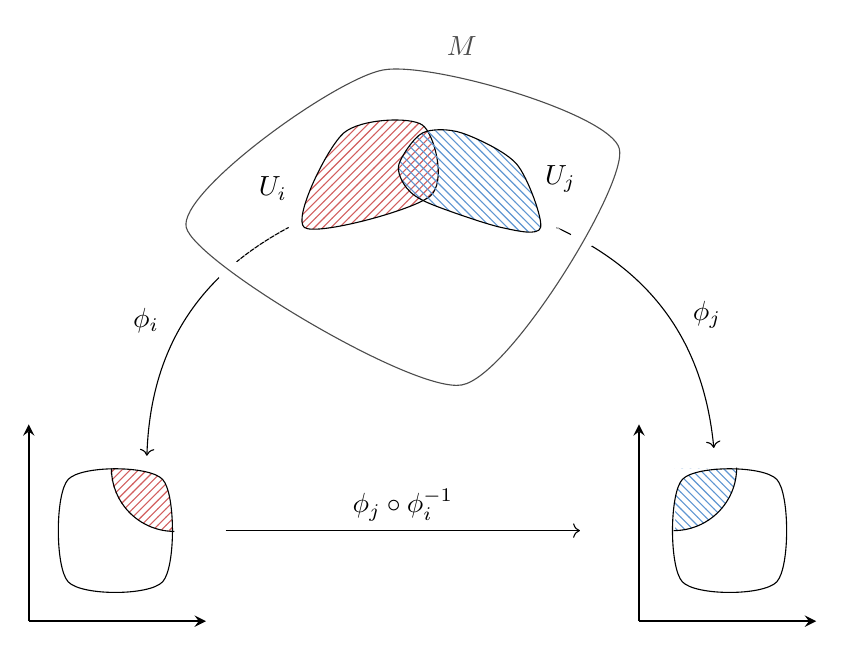
\begin{tikzpicture}[scale=1,]
               \path[->] (0.8, 0) edge [bend right] node[left, xshift=-2mm] {$\phi_i$} (-1, -2.9);
               \draw[white,fill=white] (0.06,-0.57) circle (.15cm);

               \path[->] (4.2, 0) edge [bend left] node[right, xshift=2mm] {$\phi_j$} (6.2, -2.8);
               \draw[white, fill=white] (4.54,-0.12) circle (.15cm);
           
               % Manifold
               \draw[smooth cycle, tension=0.4, fill=white, pattern color=white, pattern=north west lines, opacity=0.7] plot coordinates{(2,2) (-0.5,0) (3,-2) (5,1)} node at (3,2.3) {$M$};
           
               % Help lines
               %\draw[help lines] (-3,-6) grid (8,6);
           
               % Subsets
               \draw[smooth cycle, pattern color=BrightRed1, pattern=north east lines] 
                   plot coordinates {(1,0) (1.5, 1.2) (2.5,1.3) (2.6, 0.4)} 
                   node [label={[label distance=-0.3cm, xshift=-2cm, fill=white]:$U_i$}] {};
               \draw[smooth cycle, pattern color=BrightBlue1, pattern=north west lines] 
                   plot coordinates {(4, 0) (3.7, 0.8) (3.0, 1.2) (2.5, 1.2) (2.2, 0.8) (2.3, 0.5) (2.6, 0.3) (3.5, 0.0)} 
                   node [label={[label distance=-0.8cm, xshift=.75cm, yshift=1cm, fill=white]:$U_j$}] {};
           
               % First Axis
               \draw[thick, ->, >=stealth] (-2.5,-5) -- (-0.25, -5);
               \draw[thick, ->, >=stealth] (-2.5,-5) -- (-2.5, -2.5);
           
               % Arrow from i to j
               \draw[->] (0, -3.85) -- node[midway, above]{$\phi_j \circ \phi_i^{-1}$} (4.5, -3.85);
           
               % Second Axis
               \draw[thick, ->, >=stealth] (5.25, -5) -- (7.5, -5);
               \draw[thick, ->, >=stealth] (5.25, -5) -- (5.25, -2.5);
           
               % Sets in R^m
               \draw[white, pattern color=BrightRed1, pattern=north east lines] (-0.67, -3.06) -- +(180:0.8) arc (180:270:0.8);
               \fill[even odd rule, white] [smooth cycle] plot coordinates{(-2, -4.5) (-2, -3.2) (-0.8, -3.2) (-0.8, -4.5)} (-0.67, -3.06) -- +(180:0.8) arc (180:270:0.8);
               \draw[smooth cycle] plot coordinates{(-2, -4.5) (-2, -3.2) (-0.8, -3.2) (-0.8, -4.5)};
               \draw (-1.45, -3.06) arc (180:270:0.8);
           
               \draw[white, pattern color=BrightBlue1, pattern=north west lines] (5.7, -3.06) -- +(-90:0.8) arc (-90:0:0.8);
               \fill[even odd rule, white] [smooth cycle] plot coordinates{(7, -4.5) (7, -3.2) (5.8, -3.2) (5.8, -4.5)} (5.7, -3.06) -- +(-90:0.8) arc (-90:0:0.8);
               \draw[smooth cycle] plot coordinates{(7, -4.5) (7, -3.2) (5.8, -3.2) (5.8, -4.5)};
               \draw (5.69, -3.85) arc (-90:0:0.8);    
            \end{tikzpicture}
            \caption{Exemple de deux cartes}
      \end{figure} 
   \section{Atlas et variétés}
      On apelle alors \textbf{atlas} de \( M \) une famille \(\mathcal{A} = (U_i, \phi_i)_{i \in I}\) de cartes locales qui recouvrent \( M \) et qui sont compatibles. En outre on définit:
      \begin{itemize}
         \item Si \( \phi_{ij} \) est un homéomorphisme, on dit que l'atlas est topologique et que \( M \) est une \textbf{variété topologique}.
         \item Si \( \phi_{ij} \) est différentiable, on dit que l'atlas est différentiel et que \( M \) est une \textbf{variété différentielle}.
         \item Si \( \phi_{ij} \) est de classe \( \mathcal{C}^k \), on dit que l'atlas est de classe \( \mathcal{C}^k \) et que \( M \) est une variété de classe \( \mathcal{C}^k \).
      \end{itemize}
      Dans le cas particulier \( k = \infty \), on dira usuellement que l'atlas et la variété sont \textbf{lisses}.     
   \section{Topologie d'une variété}
   De manière générale, on définit les propriétés topologiques d'une variété par ses propriétés en tant qu'espace topologique, donc naturellement:
      \begin{itemize}
         \item On dira alors que \( M \) est \textbf{compacte} si l'espace topologique sous-jaçent l'est.
         \item On dira alors que \( M \) est \textbf{connexe} si l'espace topologique sous-jaçent l'est.
         \item On peut donc parler d'intérieur, d'adhérence d'une partie de \( M \), etc ...
         \item ...
      \end{itemize}
\chapter{Variétés à bord}
   On veut alors pouvoir relaxer cette définition pour prendre en compte une catégorie plus large d'espaces topologiques, en particulier si on considère le disque ouvert \( D^1 \), c'est trivialement\footnote[1]{Comme graphe d'une fonction constante définie sur un ouvert.} une variété, mais le disque fermé \( \text{adh}(D^1) \) ne l'est pas. La différence fondamentale étant qu'un ouvert qui contient un point du bord du disque fermé n'est pas homéomorphe à un ouvert de \( \R^2 \) Mais à un ouvert du demi-plan \( \R \times \R_+ \).

   \section{Bord du demi-espace \( \R^n_+ \)}
   On note \( \R^n_+ := \left\{ x \in \R^n  \; ; \; x_n \geq 0\right\} \). Cet espace sera notre prototype de partie avec un bord, en effet si on considère cet espace en tant que partie de \( \R^n \), son bord est bien défini:
   \[ 
      \partial \R^n_+ := \R^n_+ \backslash \text{int}(\R^n_+) = \left\{ x \in \R^n \; ; \; x_n = 0\right\}  
   \]
   Par exemple dans le cas de \( \R^2_+ \), on a:
      \begin{figure}[ht!]
         \centering
         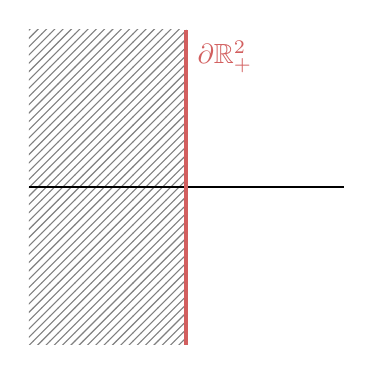
\begin{tikzpicture}
            % Hachures pour x < 0
            \fill[pattern=north east lines, pattern color=black!50] (-2,-2) rectangle (0,2);
            
            \draw[line width = 0.8] (-2,0) -- (2,0);
            \draw[color=BrightRed1, line width = 1.5] (0,-2) -- (0,2) node[below right] {$\partial \mathbb{R}^2_+$};
            \draw[color=BrightRed1, line width = 1.5] (0,-2) -- (0,2);
        \end{tikzpicture}
        \caption{Le demi plan \( \R^2_+ \) et son bord}
      \end{figure}
   \vspace{-15pt}
   \section{Variété à bord}
   On donne élargit alors notre définition d'une variété, qui sera notre définition générale pour la suite. On se donne une variété \( M \) muni de son atlas \( (U_i, \phi_i)_{i \in I} \) et on rajoute la contrainte suivante sur les cartes:
   \[ 
      \forall i \in I \; ; \; \phi_i : U_i \longmapsto V_i \text{ avec } V_i \text{ un ouvert de } \R^n_+
   \]
   Ceci nous permet de définir le bord d'une variété par:
   \[ 
      \partial M := \left\{ x \in M  \; ; \; \forall (U_i, \phi_i) \in \mathcal{A} \; ; \; x \in U_i \implies \phi_i(x) \in \partial\R^n_+\right\}  
   \]
   Alors on peut montrer que c'est bien une généralisation du concept de variété, en effet si une variété définie de la sorte n'a pas de bords, ie si \( \partial M = \emptyset\), alors on peut construire un atlas au sens du chapitre 2.\<

   En particulier, on peut remarquer que \( \R^n_+ \) lui-même est bien une variété à bord ce qui est bien cohérent ...
\chapter{Exemples de variétés}
   Dans ce chapitre, on présente quelques exemples simples de variétés différentielles, leurs atlas et quelques unes de leurs propriétés.
   \section{Le cercle \( S^1 \)}
   \section{La sphere \( S^2 \)}
   \section{Plan projectif \( \R P^2 \) ?}
\chapter{Espaces tangents}
On aimerait alors pouvoir généraliser la notion \textbf{d'espace tangent} à une courbe, surface ... lisse de \( \R^n \) à des variétés abstraites comme définies dans les deux premiers chapitres. Pour ce faire, il est fondamental de comprendre que les variétés ainsi définies ne sont \textbf{pas} des objets de \( \R^k \) et donc on doit définir cette notion purement intrinséquement, via l'atlas notamment.

\section{Courbe sur une variété}
On définit la notion de \textbf{courbe paramétrée} sur une variété \( M \) par la donnée d'une application \( \gamma : I \longmapsto M \) par exemple si on considère la sphère unité \(\mathbb{S}^2 \backslash N\) paramétrée par l'inverse de la projection stéréographique qu'on notera \( S(u, v) \), alors l'application suivante est une courbe sur la sphère:
\[ 
   \gamma : t \in \ioo{0}{1} \longmapsto S(2t^3, t^2)
\]
\section{Vecteur tangent}
On se donne une courbe \( \gamma :  I \rightarrow M\) dérivable et un réel \( t_0 \in I \), alors on veut définir le \textbf{vecteur tangent} à la courbe \( \gamma \) au point \( x = \gamma(t_0) \), pour ceci on utilise les cartes, en effet on dire que \( u \in \R^n \) est tangent à la courbe en \( x \) si et seulement si:
\[ 
   \forall (U_i, \phi_i) \in \mathcal{A} \; ; \; x \in U_i \implies u \sim (\phi_i \circ \gamma)'(t_0) 
\]
Le problème étant que ceci dépends de la carte car si le vecteur tangent à la courbe est unique, sa \textbf{représentation} (ou encore ses \textbf{coordonées}) dans les cartes ne l'est pas (elle varie avec \( d\phi_{ij} \)) donc ça marche pas ... Impossible de définir uniquement le vecteur tangent à une courbe ?!
\section{Courbes tangentes}
On fixe un point \( x \in M \) et on veut maintenant définir un espace vectoriel associé à ce point, qui correspondrait aux vecteurs tangents à la variété en ce point. Pour ceci, on définit une relation d'équivalence sur les courbes sur \( M \), en particulier, pour deux courbes paramétrées \( \gamma_1, \gamma_2 \) sur \( M \) telles que \( \gamma_1(t_0) = \gamma_2(t_0) = x \). Alors on définit:
\[ 
   \gamma_1 \sim \gamma_2 \iff \forall (U_i, \phi_i) \in \mathcal{A} \; ; \; x \in U_i \implies (\phi_i \circ \gamma_1)'(t_0) = (\phi_i \circ \gamma_2)'(t_0)
\]
On remarque tout d'abord que les hypothèse peuvent être affaiblies, en effet si la propriété est vraie pour \textbf{une carte} \( (U_i, \phi_i) \), alors par changement de carte on a que: ?\<


On obtient donc la définition suivante:
\[ 
   \gamma_1 \sim \gamma_2 \iff \exists (U, \phi) \in \mathcal{A} \; ; \; x \in U \text{ et } (\phi \circ \gamma_1)'(t_0) = (\phi \circ \gamma_2)'(t_0)
\]
C'est bien une relation d'équivalence sur l'ensemble des courbes de \( M \) qui passent par \( x \), on appelle une classe d'équivalence pour cette relation \textbf{vecteur tangent} à la courbe en \( x \) et l'ensemble quotient est donc \textbf{l'ensemble des vecteurs tangents} ou plus formellement \textbf{l'espace tangent} au point \( x \) définit par:
\[ 
   TM_x := \left\{ [\gamma] \in \mathcal{F}(I, \R) \; ; \;   \right\}  
\]
\<
Il faut maintenant montrer:
\begin{itemize}
   \item Que c'est bien un e.v (sous-ev ? Le neutre ?) de dimension \( n \).
   \item Définir la différentielle d'une application de \( M \longmapsto N \).
   \item Montrer que celle ci est bien définie sur les espaces tangents.
   \item Propriétés algèbriques, règle de la chaine etc...
\end{itemize}
   \pagebreak   
   \chapter{Algèbre extérieure dans \( \R^n \)}
\chapter{Algèbre extérieure sur une variété}
\chapter{Dérivée extérieure}
\chapter{Exactitude \& Fermeture}

   \pagebreak   
   \chapter{Intégrale d'une forme dans \( \R^n \)}
\chapter{Intégrale d'une forme sur une variété}
\chapter{Théorème de Stokes-Cartan}


   \pagebreak  
   \chapter{Applications de la théorie des formes}
   \section{Cas de la dimension 3}
   Dans le cas de \(\R^3\), on a la chaîne suivante:
   \[
      \Lambda^0 \R^3 \overset{d_0}{\longrightarrow} \Lambda^1 \R^3 \overset{d_1}{\longrightarrow} \Lambda^2 \R^3 \overset{d_2}{\longrightarrow} \Lambda^3 \R^3
   \]
   On peut alors montrer facilement que les dimensions des différents espaces suivent la suite \((1, 3, 3, 1)\) et les propriétés surprenantes suivantes:
   \begin{itemize}
      \item On a \(d_0\) qui s'identifie \textbf{au gradient de la fonction}.
      \item On a \(d_1\) qui s'identifie \textbf{au rotationnel du champ de vecteurs}.
      \item On a \(d_2\) qui s'identifie \textbf{à la divergence du champ de vecteurs}.
   \end{itemize}
   Et par la propriété fondamentale de la dérivée extérieure, on a alors les formules classiques suivantes comme simple conséquence:
   \[
      \begin{cases}
         \text{rot}(\nabla f) = 0\\
         \text{div}(\text{rot}(F)) = 0\\
      \end{cases}
   \]

\chapter{Applications du théorème de Stokes-Cartan}

   \pagebreak  
   \input{../VI-conclusion.tex}
   \pagebreak    
\end{document}
